\section{Driver Amplifier}

First, the Driver Amplifier was built. The associated schematic can be
seen in Figure~\ref{DriverAmp}.

\begin{figure}[h!]
  \centering
  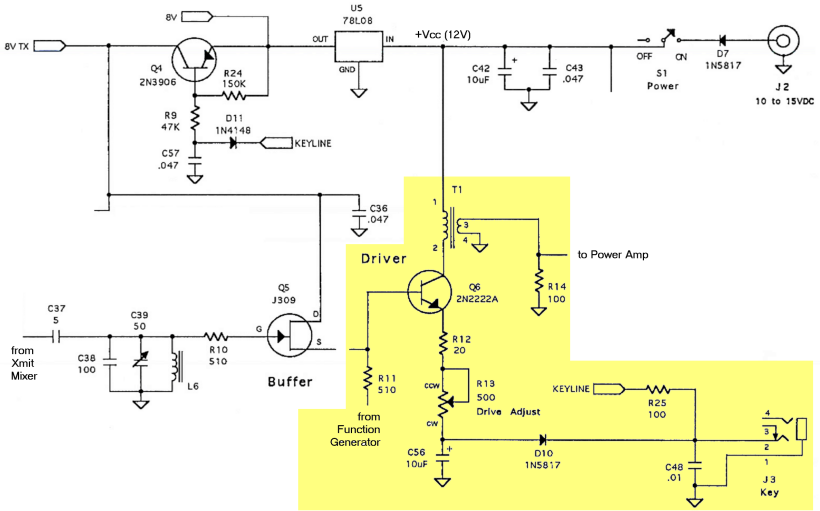
\includegraphics[scale=0.6]{./img/DriverAmp.png}
  \label{DriverAmp}
  \caption{Circuit Schematic for the Driver Amplifier}
\end{figure}

\subsection{Calculated Output Power: \bm{$P_{o}$}}
  $P_o$ is calculated using the following:

  \begin{align*}
    P_o &= \frac{V_{cc}^2}{n^2 R_{14}}\\
  \end{align*}
  Since $V_{cc}$ is given as $12V$, $R_{14} = 100 \Omega$ and transformer $T_1$ has a turns ratio $n =
  \frac{14}{4} = 3.5$:
  \begin{align*}
    P_o &= \frac{12^2}{(3.5^2 \cdot 100}i) = \boxed{117.5 mW}
  \end{align*}
\subsection{Measured Output Voltage: \bm{$V_o$}}
With the function generator set to 7.04MHz, and with an offset of 
%Remember to edit this if any changes are made!
$0.5V$. The output voltage across $R_{14}$ was measured to be $\boxed{ V}$.

\subsection{Calculated Delivered Power: \bm{$P_{d}$}}
\subsubsection{ } 
  First, the DC voltage across $R_12$ was recorded to be $\boxed{ V}$.
  \subsubsection{ }
\subsection{System Efficiency: \bm{$\eta$}}

\subsection{Amplifier Gain: \bm{$G$}}

\subsubsection{}
When $R_{13}$ is fully clockwise, the gain was found to be 
$\boxed{}$.
\subsubsection{}
When $R_{13}$ is fully counter-clockwise
$\boxed{}$.

\subsection{Miller Capacitance, \bm{$C_M$}}

(\emph{Note:} At the end of this step, the other end of $R_{11}$ was soldered).
